\section{Standardized Development Results}

The full $2^6$ observation grid generated 40,960 trajectories in 512 generator-condition cells using fresh seed blocks. Of these attempts, 2,432 lacked enough retained observations for the required split, leaving 38,528 evaluable trajectories. These attempts remain unsuccessful recovery in attempted-run summaries. There were also 672 candidate-level rank-deficient fits; candidate failures are distinct from trajectory failures and are not an additional number of excluded trajectories. These are developmental results registered as \texttt{M02-DEV-FACTORIAL-2026-10-07}.

\begin{table}[htbp]
\centering
\caption{Standardized development benchmark: nominal recovery}
\label{tab:m02-standardized-development}
\begin{tabular}{lrrr}
\toprule
Generator & Reference & Analyst noise & Combined \\
\midrule
intercept & 17/80 & 12/80 & 12/80 \\
ar & 42/80 & 46/80 & 4/80 \\
p & 15/80 & 4/80 & 1/80 \\
pi & 47/80 & 29/80 & 8/80 \\
pid & 79/80 & 41/80 & 4/80 \\
arx & 80/80 & 77/80 & 9/80 \\
nonlinear & 78/80 & 24/80 & 16/80 \\
switching & 79/80 & 40/80 & 11/80 \\
\bottomrule
\end{tabular}
\end{table}


In the referent condition (180 steps, stride 1, no analyst noise or gaps, $b=0.5$, $A=1$), nominal PID recovery was 79/80, with Wilson 95\% interval approximately 0.933--0.998. At analyst-noise SD 0.04, it fell to 41/80 (approximately 0.405--0.619). Combined adversity used 60 steps, stride 3, noise SD 0.04, MCAR probability 0.25, feedback 0.1 and action bound 0.025. PID recovery was 4/80 attempts, or 4/42 evaluable trajectories. Reporting only the latter denominator would conceal observation-design infeasibility.

Recovery also varied substantially across generators within the reference arm: P was selected in 15/80 attempts and the intercept-only generator in 17/80, compared with 79/80 for PID. The candidate set contains richer regressions that include lower-order behavior as a special case. Unpenalized validation RMSE can therefore favor a richer family even when the nominal generator is simpler. Exact nominal recovery is a demanding label-level criterion; these counts cannot by themselves establish that P-like behavior is poorly predicted. Confusion matrices and effective-order scores complement nominal recovery, and a uniform chance rate is inappropriate for this nested set.

Combined adversity did not universally favor the simplest baselines. For nominal PID in that arm, the selected families included nonlinear in 13 cases, PI in 10 and ARX in 7, but intercept in only 2 and AR in none; 38 attempts failed the observation split. Family confusion and design failure therefore require separate interpretation.

Strong nominal discrimination did not guarantee a material predictive advantage at the chosen development resolution. Reference PID's mean paired final-test RMSE difference against its validation-selected competitor was approximately $-0.000841$, with pointwise 95\% normal interval $[-0.000957,-0.000725]$. This interval excludes zero but remains inside the development band $[-0.005,0.005]$. Statistical separation from zero and practical predictive equivalence therefore coexist at this resolution; neither conclusion is structural equivalence or evidence about people.

Across the 512 cells, 405 paired mean intervals were wholly inside the development band, 74 were inconclusive, 23 favored the nominal generator beyond the band and 10 favored the competitor beyond it. These are pointwise development descriptions rather than multiplicity-controlled confirmatory decisions. Short/sparse adverse conditions can produce unstable candidate extrapolation and very broad intervals; the normal approximation and fixed numerical tolerance require further calibration before final inferential claims.

The separate targeted benchmark generated 5,760 trajectories with a different seed pool. Its exact-reduction condition gives the nominal PID generator zero integral and derivative gains. This produces actions identical to P under matched noise. Nominal PID was selected in 14/80 cases while effective P was selected in 20/80. The discrepancy between those scores is a labeling issue, not recoverable evidence for distinct mechanisms. The targeted study is registered separately as \texttt{M02-DEV-STANDARDIZED-2026-10-07}; it is not pooled with the factorial grid.

\begin{figure}[htbp]
\centering
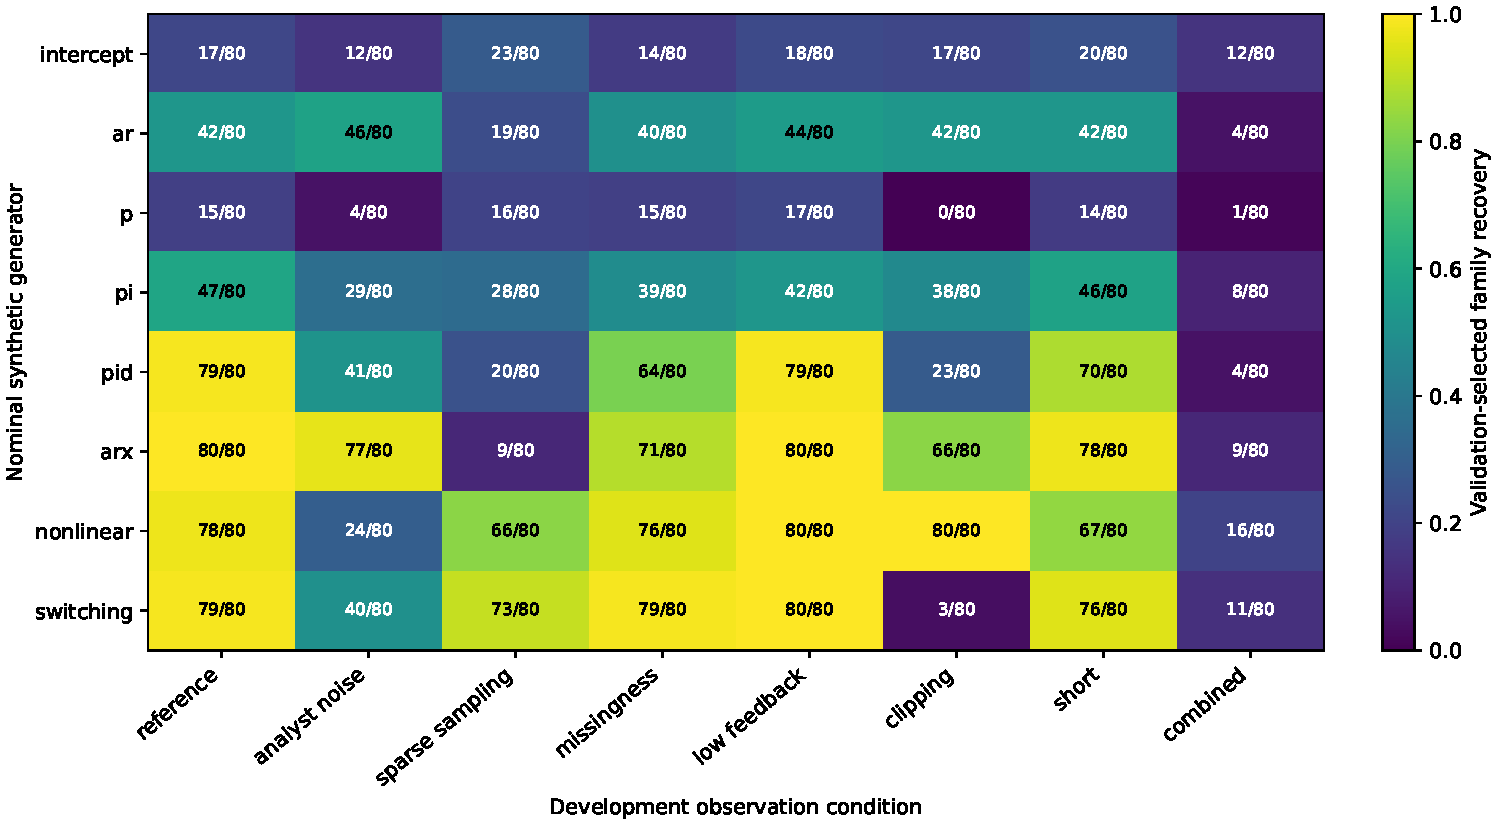
\includegraphics[width=\linewidth]{figures/m02_development_recovery.pdf}
\caption{Nominal generator recovery in eight displayed observation arms of the full development grid. Counts retain all 80 attempts per cell, including failed trajectory splits. Colors show validation-selected recovery, not psychological validity. The complete 64-condition summaries and Wilson intervals are archived separately.}
\label{fig:m02-development-recovery}
\end{figure}

\begin{figure}[htbp]
\centering
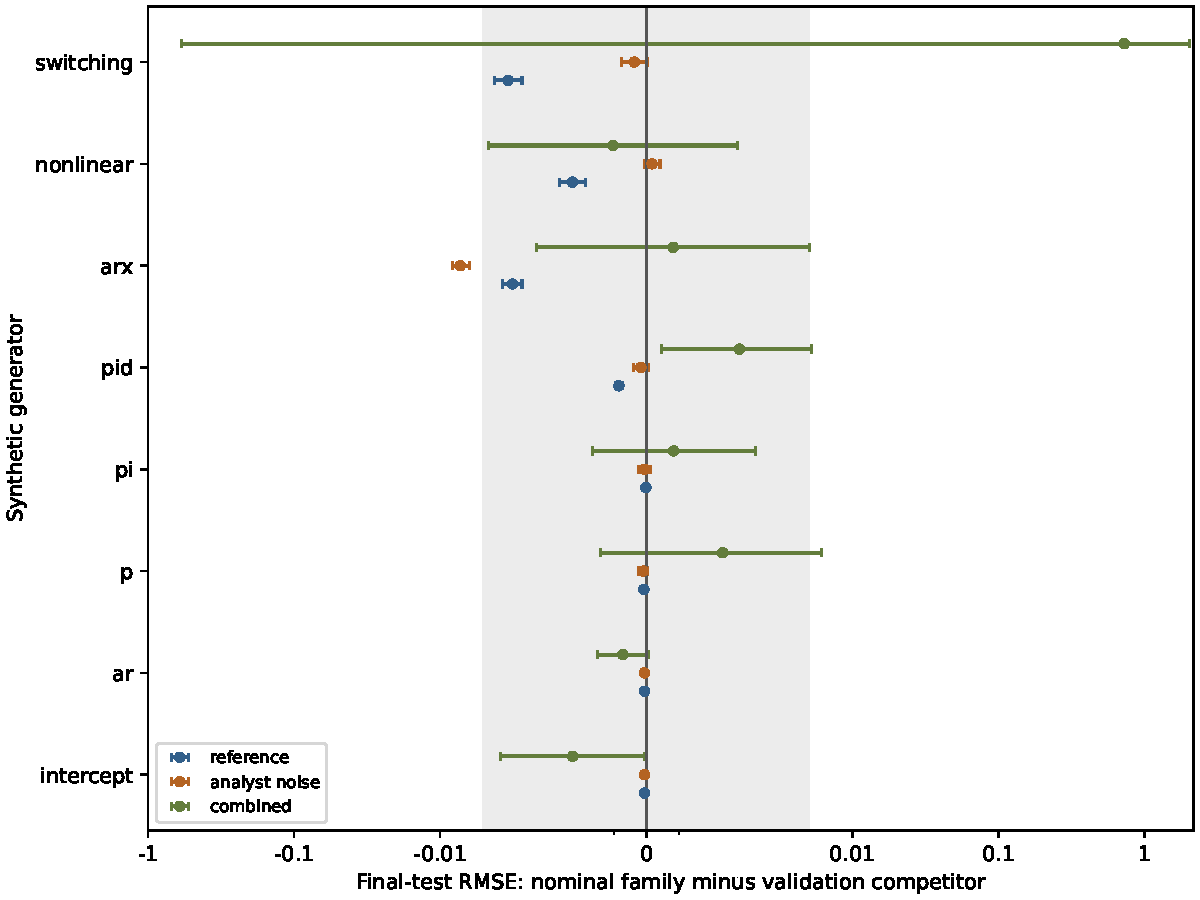
\includegraphics[width=0.90\linewidth]{figures/m02_development_paired_loss.pdf}
\caption{Paired final-test RMSE differences for three development arms. Negative values favor the fitted nominal family; positive values favor the competitor chosen on validation excluding that family. Pointwise 95\% normal intervals use evaluable paired trajectories, with counts in the archived summary. The shaded band is the fixed development tolerance; the horizontal axis is symmetric logarithmic outside its central linear region. Broad intervals are inconclusive rather than evidence of equality.}
\label{fig:m02-development-paired-loss}
\end{figure}

All generators use fixed gains, and nonlinear width and switching boundary are known. The plant deliberately simplifies the historical ARC-inspired agent. MCAR gaps, conditional action prediction and noisily reconstructed histories limit transfer beyond these settings. Parameter bias/dispersion are archived for evaluable nominal-family fits, without implemented coverage intervals. Neither development experiment substitutes for a frozen, independently reproduced final computational protocol.
